\chapter{نتایج و تحلیل خطا}
\label{ch:results}

این فصل سه مرحله کار را به ترتیب می‌آورد: شش تکرار روی زیرمجموعه $50$ سندی، اجرای کامل روی $500$ سند، و در پایان پیکره کامل \lr{DocRED}.

\section{شش تکرار روی زیرمجموعه}
\label{sec:six-versions}

زیرمجموعه $50$ سند نخست بخش \lr{Dev} است با $1{,}868$ سه‌تایی طلایی و $85$ رابطه متمایز. مدل \lr{gpt-4.1-mini} با دمای صفر. جدول \ref{tab:six} شش نسخه را نشان می‌دهد.

\begin{table}[ht]
\centering
\caption{شش تکرار روی زیرمجموعه $50$ سندی.}
\label{tab:six}
\begin{adjustbox}{max width=\textwidth}
\small
\begin{tabular}{|r|r|c|c|c|c|c|}
\hline
نسخه & توضیح & سه‌تایی & دقت & بازخوانی & $F_1$ & $\mathrm{Ign}\,F_1$ \\
\hline
\lr{v1} & پرامپت پایه & $466$ & $42.27$ & $10.55$ & $16.88$ & $19.20$ \\
\hline
\lr{v2} & پرامپت جامع با استنتاج و رابطه معکوس & $716$ & $36.45$ & $13.97$ & $20.20$ & $21.06$ \\
\hline
\lr{v3} & \lr{v2} به‌علاوه لایه بستار & $985$ & $34.11$ & $17.99$ & $23.55$ & $23.90$ \\
\hline
\lr{v4} & \lr{v2} به‌علاوه دو مثال کاری & $501$ & $45.11$ & $12.10$ & $19.08$ & $19.86$ \\
\hline
\lr{v5} & \lr{v4} به‌علاوه لایه بستار & $710$ & $45.35$ & $17.24$ & $24.98$ & $25.52$ \\
\hline
\lr{v6} & اجماع سه گذر به‌علاوه لایه بستار & $1{,}531$ & $32.92$ & $26.98$ & $29.66$ & $29.35$ \\
\hline
\end{tabular}
\end{adjustbox}
\end{table}

چیزی که از این جدول یاد گرفتیم، برخلاف انتظار اولیه‌مان بود. تصور ما این بود که گذاشتن مثال در پرامپت بازخوانی را بالا می‌برد، چون مدل بهتر می‌فهمد چه می‌خواهیم. اما مقایسه \lr{v2} با \lr{v4} عکس این را نشان داد: دقت از $36.45$ به $45.11$ رفت، یعنی $24\%$ رشد نسبی، و در همان حال تعداد خروجی کمتر شد. وقتی نرخ رد شدن توسط فیلتر هستان‌شناسی را نگاه کردیم دلیلش روشن شد؛ این نرخ از $20.3\%$ به $18.7\%$ افتاده بود، یعنی مدل از همان اول کمتر رابطه نامعتبر می‌ساخت.

لایه بستار روی هر دو پرامپت جواب داد، که خیالمان را راحت کرد: از \lr{v2} به \lr{v3} مقدار $F_1$ را $3.35$ واحد و از \lr{v4} به \lr{v5} آن را $5.90$ واحد بالا برد. یعنی کارش وابسته به یک پرامپت خاص نبود.

بزرگ‌ترین جهش اما از جای دیگری آمد. سه گذر مستقل با پرامپت‌های متفاوت، مجموعه‌های متفاوتی از حقیقت‌ها پیدا می‌کنند و اجتماع ساده آن‌ها بازخوانی را از $17.24$ به $26.98$ و $F_1$ را به $29.66$ رساند. برداشت ما از این عدد این است که گلوگاه سامانه هیچ‌وقت ندانستن مدل نبود، کم‌گویی‌اش در یک گذر واحد بود.

یک نکته دیگر هم در این جدول هست که به‌راحتی از چشم می‌افتد. مقدار $\mathrm{Ign}\,F_1$ در همه نسخه‌ها نزدیک $F_1$ یا حتی بالاتر از آن مانده. این یعنی امتیازی که می‌گیریم از حافظه پیش‌آموخته مدل نمی‌آید و مدل واقعاً دارد متن سند را می‌خواند.

\section{سهم لایه بستار}
\label{sec:closure-share}

در \lr{v3} این لایه $270$ حقیقت ساخت که $153$ تا از قاعده وارون، $104$ تا از تراگذری و $13$ تا از زنجیره آمد. از این $270$ مورد، $76$ مورد در پاسخ طلایی هم بود، یعنی دقت $28.1\%$. این از دقت خود مدل زبانی پایین‌تر است، پس لایه قاعده در عمل بازخوانی می‌خرد و بخشی از دقت را می‌فروشد. چون $F_1$ کل در هر شش نسخه بالا رفت، این معامله را به سود خودمان دیدیم.

\section{اجرای کامل روی پانصد سند}
\label{sec:full-dev}

جدول‌های بالا همه روی زیرمجموعه $50$ سند بودند و این نگرانی را داشتیم که عدد به یک نمونه کوچک وابسته باشد. برای همین سامانه را روی کل $500$ سند بخش \lr{Dev} اجرا کردیم: $17{,}284$ سه‌تایی طلایی، $95$ رابطه متمایز و $1{,}000$ فراخوانی مدل زبانی در دو گذر. نتیجه در جدول \ref{tab:full500} آمده است.

\begin{table}[ht]
\centering
\caption{اجرای کامل روی هر $500$ سند بخش \lr{Dev} با برچسب بازبینی‌شده \lr{Re-DocRED}.}
\label{tab:full500}
\small
\begin{tabular}{|r|c|c|c|c|c|}
\hline
نسخه & سه‌تایی & دقت & بازخوانی & $F_1$ & $\mathrm{Ign}\,F_1$ \\
\hline
گذر \lr{A} بدون مثال & $6{,}176$ & $36.84$ & $13.16$ & $19.39$ & $19.93$ \\
\hline
گذر \lr{B} با دو مثال & $5{,}109$ & $44.63$ & $13.19$ & $20.36$ & $20.53$ \\
\hline
اجماع و بستار & $11{,}787$ & $35.32$ & $24.09$ & $28.64$ & $28.23$ \\
\hline
\end{tabular}
\end{table}

اختلاف $F_1$ بین دو مقیاس $0.56$ واحد شد، که برای خیال راحت کافی بود: عدد زیرمجموعه اتفاقی نبوده. لایه بستار در این مقیاس $3{,}251$ حقیقت استنتاجی ساخت.

\section{مرحله سوم: پیکره کامل \lr{DocRED}}
\label{sec:stage3}

تا اینجا همه آزمایش‌ها روی زیرمجموعه‌های کوچک بود. برای اجرا روی کل پیکره سه چیز را عوض کردیم و باقی پیکربندی را دست‌نخورده نگه داشتیم، یعنی همان هستان‌شناسی و همان دو مثال و همان سه قاعده، تا بشود اثر همین سه تغییر را جدا دید.

اول مدل زبانی عوض شد و به‌جای \lr{gpt-4.1-mini} از \lr{Claude Sonnet} استفاده کردیم؛ علتش هم فنی نبود، کلید پولی به سقف هزینه خورده بود. دوم، قالب پاسخ را فشرده کردیم: مدل به‌جای \lr{JSON} کامل فقط شماره موجودیت و شماره جمله را برمی‌گرداند و متن شاهد را خودمان از سند درمی‌آوریم، که طول پاسخ را حدود چهار برابر کم می‌کند. سوم، در ترکیب دو گذر به‌جای اجتماع سراغ اشتراک رفتیم.

\subsection{بخش \lr{Dev} کامل}
\label{sec:dev998}

$998$ سند با برچسب اصلی \lr{DocRED}، $12{,}275$ سه‌تایی طلایی و $96$ رابطه. جدول \ref{tab:dev998} نتیجه را می‌دهد.

\begin{table}[ht]
\centering
\caption{بخش \lr{Dev} کامل، $998$ سند، برچسب اصلی \lr{DocRED}.}
\label{tab:dev998}
\small
\begin{tabular}{|r|c|c|c|c|c|}
\hline
نسخه & سه‌تایی & دقت & بازخوانی & $F_1$ & $\mathrm{Ign}\,F_1$ \\
\hline
گذر \lr{A} بدون مثال & $13{,}769$ & $32.57$ & $36.53$ & $34.43$ & $34.50$ \\
\hline
گذر \lr{B} با دو مثال & $16{,}741$ & $30.64$ & $41.79$ & $35.36$ & $34.41$ \\
\hline
اشتراک دو گذر و بستار & $10{,}616$ & $39.08$ & $33.80$ & $36.25$ & $36.83$ \\
\hline
\end{tabular}
\end{table}

اینجا چیزی دیدیم که با مرحله قبل جور درنمی‌آمد. با مدل تازه، مثال دیگر دقت نمی‌خرد بلکه بازخوانی می‌خرد و آن را از $36.53$ به $41.79$ می‌رساند، و این اشتراک دو گذر است که دقت را از $32.57$ به $39.08$ می‌برد. گرفتن اشتراک خروجی را از $16{,}741$ به $10{,}616$ سه‌تایی آب می‌کند و اول فکر کردیم این حتماً به ضرر $F_1$ تمام می‌شود، ولی نشد؛ سه‌تایی‌هایی که فقط یک گذر دیده بودشان بیشترشان غلط بودند.

برای مقایسه، همان $998$ سند با \lr{gpt-4.1-mini} و اجتماع دو گذر $F_1$ برابر $21.38$ گرفته بود.

\subsection{همان پیش‌بینی، دو مجموعه برچسب}
\label{sec:two-labels}

$498$ سند از این $998$ سند، همان سندهای بخش \lr{Dev} مرحله قبل‌اند. پس می‌شود یک مجموعه پیش‌بینی ثابت را یک بار با برچسب اصلی \lr{DocRED} و یک بار با برچسب بازبینی‌شده \lr{Re-DocRED} سنجید. جدول \ref{tab:two-labels} همین است.

\begin{table}[ht]
\centering
\caption{یک مجموعه پیش‌بینی ثابت روی $498$ سند مشترک، سنجیده‌شده با دو مجموعه برچسب.}
\label{tab:two-labels}
\small
\begin{tabular}{|r|c|c|c|c|c|}
\hline
برچسب طلایی & سه‌تایی طلایی & دقت & بازخوانی & $F_1$ & $\mathrm{Ign}\,F_1$ \\
\hline
\lr{DocRED} اصلی & $6{,}141$ & $40.20$ & $33.72$ & $36.68$ & $37.22$ \\
\hline
\lr{Re-DocRED} بازبینی‌شده & $17{,}183$ & $66.42$ & $19.92$ & $30.64$ & $31.66$ \\
\hline
\end{tabular}
\end{table}

برچسب‌های بازبینی‌شده $2.8$ برابر بیشترند و دقت همان پیش‌بینی‌ها را از $40.20$ به $66.42$ می‌رسانند. یعنی حدود $40\%$ از آنچه روی برچسب اصلی «مثبت کاذب» شمرده می‌شد، در واقع رابطه‌هایی بوده که در متن هست و فقط کسی برچسبشان نزده. همان چیزی که مقاله \lr{Re-DocRED} ادعا کرده، اینجا با سامانه خودمان مستقیماً اندازه گرفته شد. برای خواندن باقی جدول‌های این گزارش یک نتیجه عملی دارد: هر عدد دقتی که روی برچسب اصلی \lr{DocRED} می‌بینید کران پایین است، نه عدد واقعی.

\subsection{بخش‌های دیگر با همان پیکربندی}
\label{sec:other-splits}

جدول \ref{tab:splits} نتیجه همه بخش‌ها را با پیکربندی قفل‌شده می‌دهد.

\begin{table}[ht]
\centering
\caption{نتیجه همه بخش‌ها با یک پیکربندی ثابت. برچسب بخش \lr{Test} در \lr{DocRED} عمومی نیست.}
\label{tab:splits}
\begin{adjustbox}{max width=\textwidth}
\small
\begin{tabular}{|r|c|c|c|c|c|c|}
\hline
بخش & سند & سه‌تایی طلایی & سه‌تایی خروجی & دقت & بازخوانی & $F_1$ \\
\hline
\lr{Dev} (\lr{DocRED}) & $998$ & $12{,}275$ & $10{,}616$ & $39.08$ & $33.80$ & $36.25$ \\
\hline
\lr{Train} برچسب‌خورده & $3{,}053$ & $38{,}180$ & $33{,}054$ & $39.14$ & $33.89$ & $36.33$ \\
\hline
\lr{Test} (\lr{Re-DocRED}) & $500$ & $17{,}448$ & $5{,}559$ & $65.61$ & $20.90$ & $31.70$ \\
\hline
\lr{Test} (\lr{DocRED}) & $1{,}000$ & \lr{--} & $10{,}676$ & \lr{--} & \lr{--} & \lr{--} \\
\hline
نظارت‌ازدور & $10{,}985$ & $160{,}555$ & $192{,}934$ & $24.23$ & $29.12$ & $26.45$ \\
\hline
\end{tabular}
\end{adjustbox}
\end{table}

مهم‌ترین چیزی که از این جدول درآمد، سطر دوم است. عدد بخش \lr{Train} برچسب‌خورده $36.33$ شد، تقریباً برابر $36.25$ بخش \lr{Dev}، آن هم با اندازه‌ای سه برابر و بدون اینکه این بخش در تنظیم پرامپت نقشی داشته باشد. برای ما این یعنی سامانه روی \lr{Dev} بیش‌برازش نشده، و نزدیک‌ترین چیزی است که بدون داشتن برچسب \lr{Test} می‌شد به یک ارزیابی بی‌طرف رسید.

سطر آخر را نباید دقت خواند؛ توافق است. بخش نظارت‌ازدور $101{,}873$ سند دارد و برچسبش ماشینی است. یک نمونه تصادفی $20{,}000$ سندی برداشتیم و گذر \lr{A} روی $10{,}985$ سند آن پیش رفت تا سهمیه هفتگی مدل تمام شد. چون خروجی در فایل کناری می‌ماند هیچ سندی دوباره خرج نمی‌شود، و همین تعداد برای نشان دادن مقیاس کافی بود. لایه بستار در این مقیاس $36{,}799$ سه‌تایی تازه ساخت و $F_1$ را از $26.13$ به $26.45$ برد.

\subsection{هزینه و توان عملیاتی}
\label{sec:cost}

همه اجراها روی یک لپ‌تاپ با چهار هسته فیزیکی و $16$ کارگر هم‌زمان انجام شد. جدول \ref{tab:cost} مصرف واقعی را می‌دهد؛ این اعداد از پاسخ خود سرویس خوانده شده‌اند و تخمین نیستند.

\begin{table}[ht]
\centering
\caption{هزینه و زمان اجرای مرحله سوم.}
\label{tab:cost}
\begin{adjustbox}{max width=\textwidth}
\small
\begin{tabular}{|r|c|c|c|c|c|}
\hline
اجرا & سند & فراخوان & توکن ورودی & توکن خروجی & زمان \\
\hline
چهار بخش برچسب‌خورده & $5{,}551$ & $11{,}190$ & $43.7$ میلیون & $3.1$ میلیون & $3.3$ ساعت \\
\hline
نظارت‌ازدور & $10{,}985$ & $10{,}287$ & $26.7$ میلیون & $2.6$ میلیون & $3.5$ ساعت \\
\hline
\end{tabular}
\end{adjustbox}
\end{table}

توان عملیاتی پایدار $49.3$ سند در دقیقه بود. گلوگاه پردازنده است و نه حافظه، چون هر کارگر حدود $170$ مگابایت بیشتر نمی‌گیرد. کش پرامپت هم کار خودش را کرد و $20.1$ میلیون توکن از $43.7$ میلیون توکن ورودی از کش آمد، چون مثال‌ها همیشه در ابتدای پرامپت و ثابت‌اند.

\subsection{گراف نهایی}
\label{sec:final-graph}

خروجی هر پنج بخش، جمعاً $16{,}536$ سند، با بارگذار دسته‌ای در \lr{Neo4j} بار شد. بارگذاری با \lr{MERGE} انجام می‌شود، پس اجرای دوباره هیچ گره یا یال تکراری نمی‌سازد. سنگین‌ترین بخش همان نظارت‌ازدور بود: $192{,}912$ رابطه در $63$ ثانیه. پایگاه در پایان $111{,}912$ گره موجودیت، $253{,}007$ یال رابطه با $101$ نوع متمایز، و $278{,}632$ گره شاهد دارد.

کشیدن $253$ هزار یال روی یک صفحه هیچ فایده‌ای ندارد، برای همین به رابط وب یک جست‌وجوی موجودیت اضافه کردیم. شکل \ref{fig:search} همسایگی \lr{Tehran} را نشان می‌دهد که $58$ موجودیت و $92$ رابطه دارد. پنل کناری جمله منبع هر رابطه را می‌آورد.

\begin{figure}[ht]
\centering
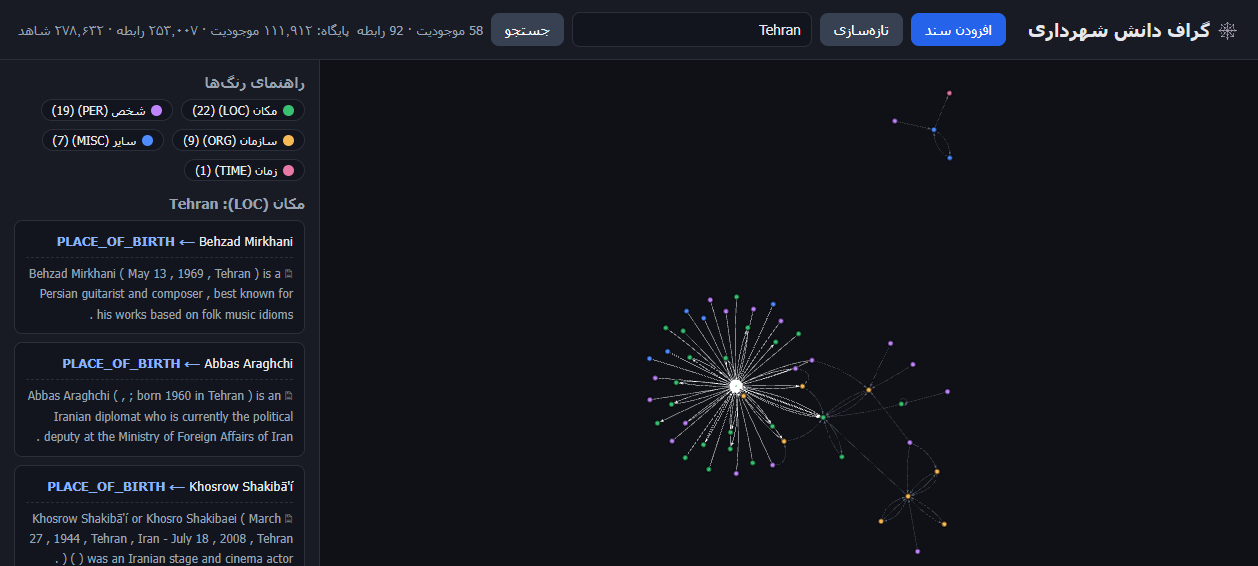
\includegraphics[width=\textwidth]{Images/graph_docred_search.png}
\caption{جست‌وجوی موجودیت در گراف $16{,}536$ سندی. سربرگ اندازه کل پایگاه و پنل کناری جمله شاهد هر رابطه را نشان می‌دهد.}
\label{fig:search}
\end{figure}

همان رابط روی خروجی \lr{Re-DocRED} هم کار می‌کند. شکل \ref{fig:neo4j} نمای مرورگر \lr{Neo4j} را بعد از بارگذاری نشان می‌دهد و شکل \ref{fig:evidence} نشان می‌دهد هر یال تا کدام جمله سند قابل ردیابی است.

\begin{figure}[ht]
\centering
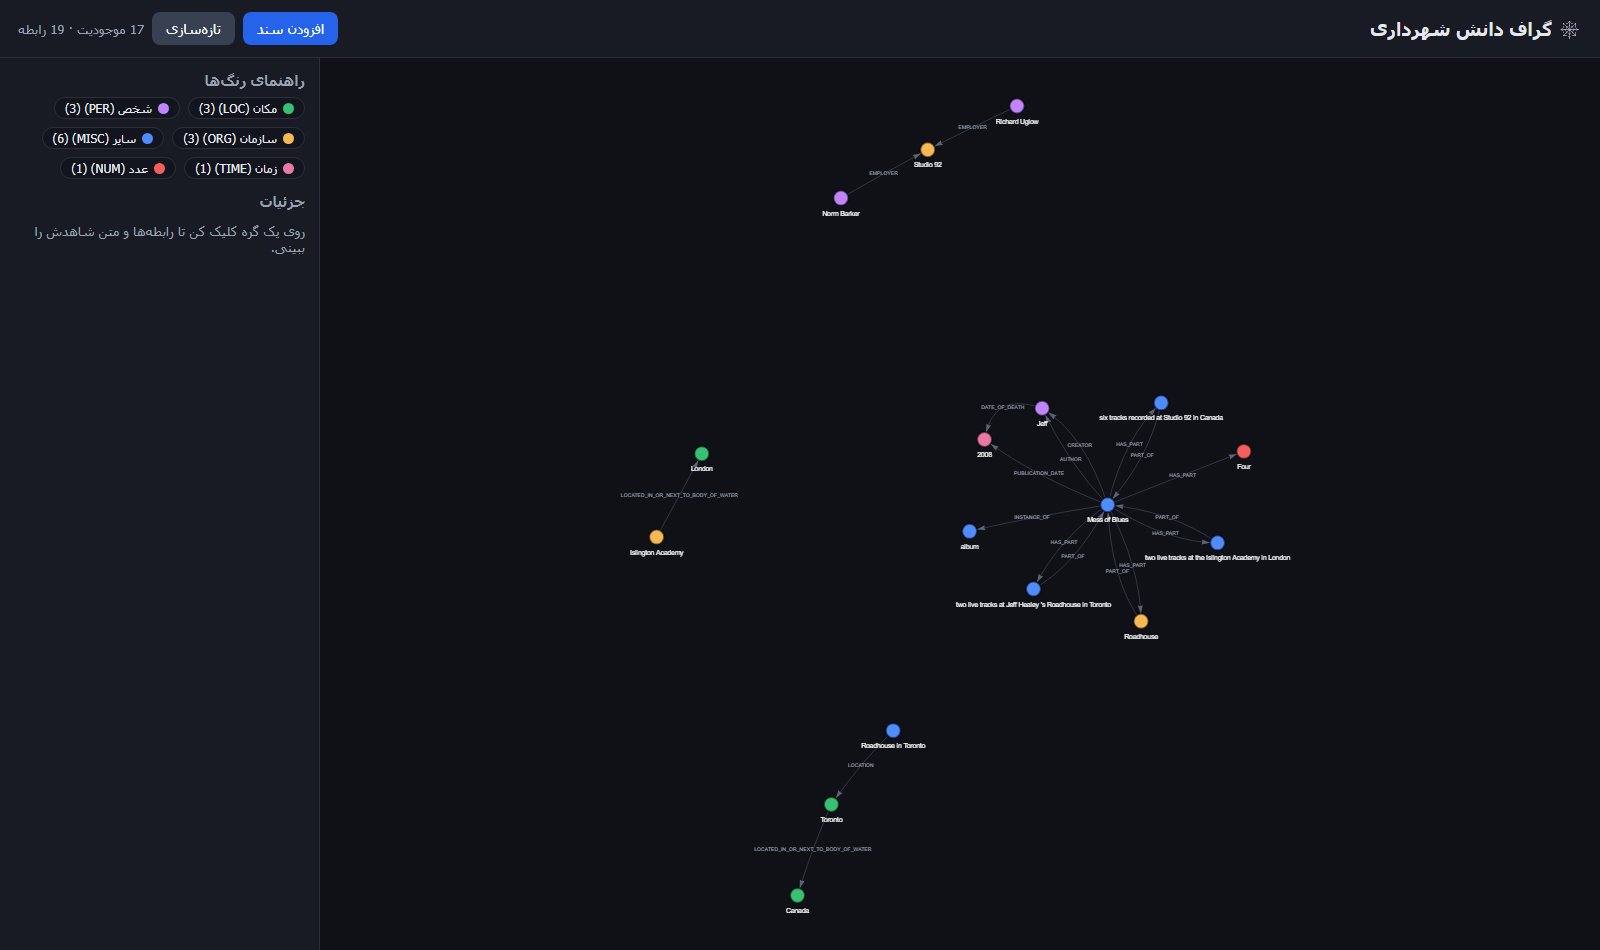
\includegraphics[width=\textwidth]{Images/graph_redocred_neo4j.png}
\caption{گراف بارگذاری‌شده در مرورگر \lr{Neo4j}. گره‌های موجودیت، یال‌های رابطه و گره‌های شاهد در یک پایگاه کنار هم می‌نشینند.}
\label{fig:neo4j}
\end{figure}

\begin{figure}[ht]
\centering
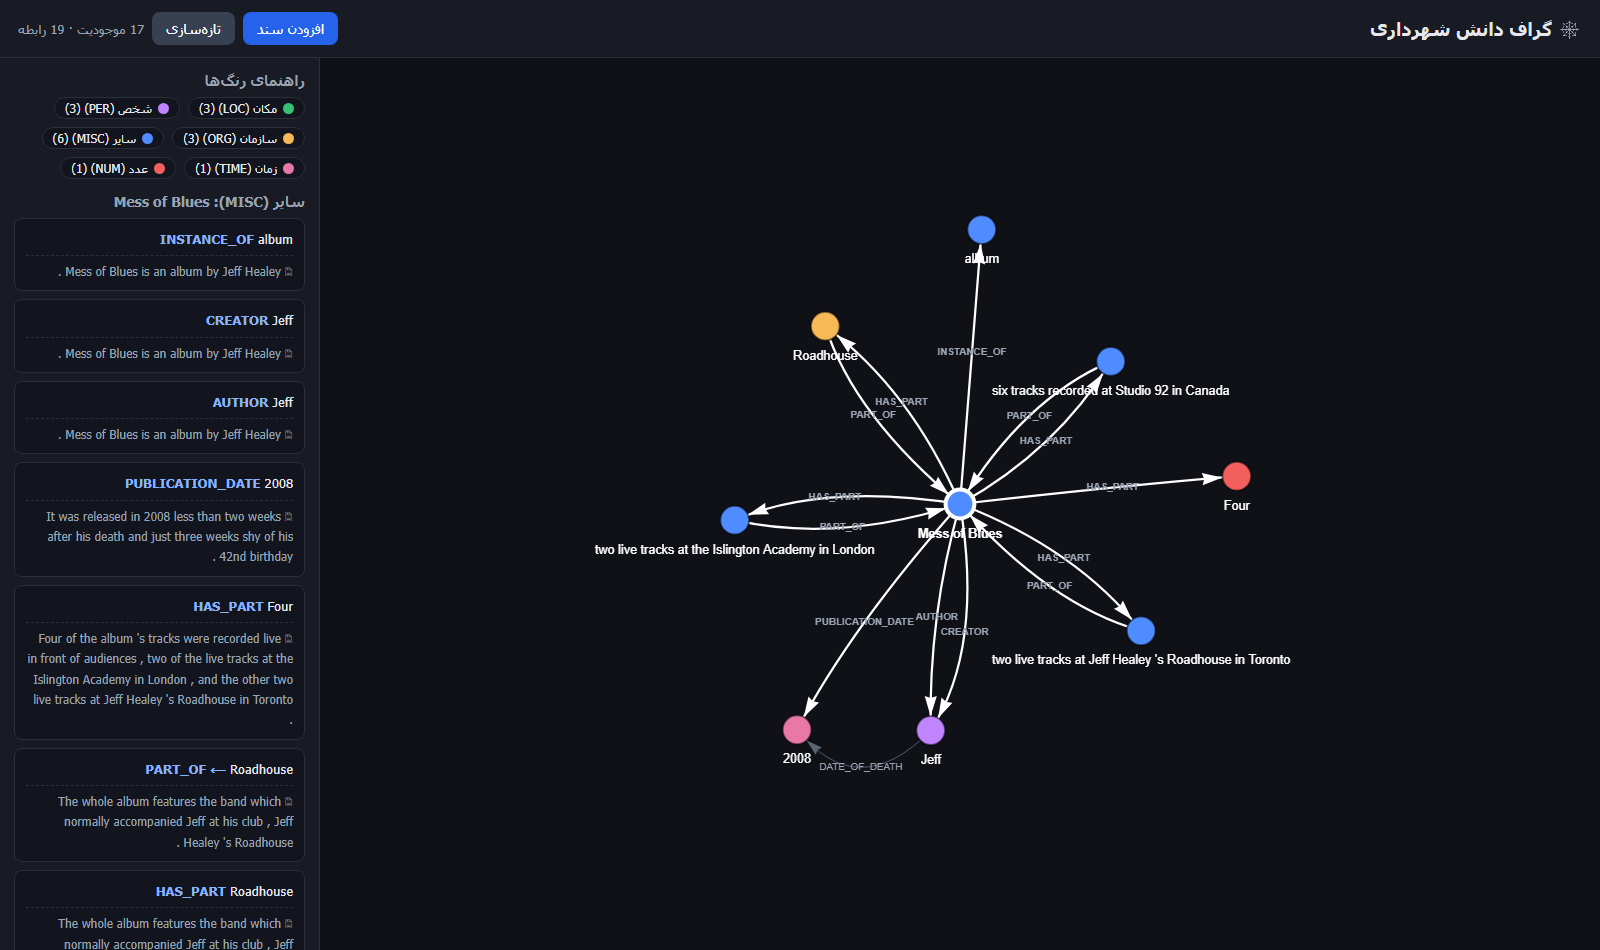
\includegraphics[width=\textwidth]{Images/graph_redocred_evidence.png}
\caption{ردیابی یک رابطه تا جمله منبع آن. هیچ یالی بدون شاهد وارد گراف نمی‌شود.}
\label{fig:evidence}
\end{figure}

\section{مقایسه با کارهای منتشرشده}
\label{sec:comparison}

جدول \ref{tab:published} کار ما را کنار نتایج منتشرشده می‌گذارد.

\begin{table}[ht]
\centering
\caption{مقایسه با کارهای منتشرشده روی \lr{Re-DocRED}.}
\label{tab:published}
\small
\begin{tabular}{|r|r|c|}
\hline
سامانه & آموزش & $F_1$ \\
\hline
\lr{KD-DocRE} \cite{kddocre} & نظارت‌شده روی $3{,}053$ سند & $81.04$ \\
\hline
\lr{ATLOP} \cite{atlop} & نظارت‌شده & $79.46$ \\
\hline
\lr{GLiDRE} \cite{glidre} & نظارت‌شده & $77.83$ \\
\hline
\lr{GPT-3.5} با \lr{NLI} \cite{gptre} & بدون آموزش و بدون مثال & $9.74$ \\
\hline
این کار (\lr{v3}) & بدون مثال، هستان‌شناسی از \lr{Train} & $23.55$ \\
\hline
این کار (\lr{v6}) & دو مثال و اجماع سه گذر & $29.66$ \\
\hline
این کار ($500$ سند \lr{Dev}) & دو مثال و اجماع دو گذر & $28.64$ \\
\hline
این کار ($500$ سند \lr{Test}) & قالب فشرده و اشتراک دو گذر & $31.70$ \\
\hline
\end{tabular}
\end{table}

حرف اصلی این جدول این است که سامانه بدون هیچ مرحله آموزش گرادیانی و فقط با دو مثال در پرامپت، بیش از سه برابر خط مبنای منتشرشده امتیاز گرفته. فاصله‌اش با مدل‌های نظارت‌شده هنوز زیاد است، ولی این فاصله را انتظار داشتیم؛ آن مدل‌ها روی سه هزار سند برچسب‌خورده آموزش دیده‌اند.

دو چیز را هنگام خواندن این جدول باید در نظر گرفت. سطر \lr{GPT-3.5} واقعاً بدون هیچ نظارتی است ولی سطرهای ما نیستند، پس مقایسه مستقیم به سود ما تمام می‌شود؛ سطر منصفانه برای چنین مقایسه‌ای \lr{v1} با $F_1$ برابر $16.88$ است. نکته دوم اینکه فقط سطر آخر روی همان بخش \lr{Test} بازبینی‌شده‌ای است که مدل‌های نظارت‌شده روی آن گزارش شده‌اند.

\section{تحلیل خطا}
\label{sec:error-analysis}

\subsection{کار مؤثر فیلتر هستان‌شناسی}
در اجرای \lr{v2} مدل زبانی $948$ سه‌تایی برگرداند و فیلتر نوع $192$ مورد، یعنی $20.3\%$، را رد کرد. پرتکرارترین ایراد چیزی بود که انتظارش را نداشتیم: معکوس بودن جهت رابطه.

\subsection{کم‌گویی، علت اصلی بازخوانی پایین}
پاسخ طلایی هر سند به‌طور میانگین $37.4$ رابطه دارد، در حالی که مدل در \lr{v1} فقط $9.3$ رابطه می‌داد و در \lr{v3} به $19.7$ رسید. الگو روشن است: مدل جمله‌های صریح را می‌بیند و از کنار حقیقت‌هایی که باید از زنجیره هم‌مرجعی یا استنتاج بیرون کشیده شوند رد می‌شود.

\subsection{نوع خطای مثبت کاذب}
از $649$ مثبت کاذب نسخه \lr{v3}، در $128$ مورد یعنی $19.7\%$ جفت‌موجودیت واقعاً رابطه دارد ولی برچسب رابطه اشتباه انتخاب شده، و در $521$ مورد یعنی $80.3\%$ جفت‌موجودیت در پاسخ طلایی هیچ رابطه‌ای ندارد. این تفکیک برایمان مهم بود، چون نوع اول با هستان‌شناسی دقیق‌تر قابل کم شدن است.

\subsection{خطای نگاشت نام}
در \lr{v6} نود سطر از $1{,}645$ سطر، یعنی $5.5\%$، به هیچ موجودیت طلایی نگاشت نشد، چون مدل نام را دقیقاً از فهرست کپی نکرده بود. همین نرخ در \lr{v3} برابر $3.6\%$ بود.

\section{ممیزی مستقل ارزیاب}
\label{sec:audit}

بعد از اینکه نتایج جمع شد، کد ارزیابی و تست‌ها را به یک مدل زبانی دیگر دادیم و از آن خواستیم علیه ادعاهای این گزارش استدلال کند. یازده ایراد گرفت که چهارتایش وارد بود و هر چهار مورد را اصلاح کردیم: کلید $\mathrm{Ign}\,F_1$ در دو بخش ناهمخوان ساخته می‌شد، تطبیق نام بیش از حد آسان‌گیر بود، گزارش خودش را «بدون نظارت» می‌نامید در حالی که هستان‌شناسی از \lr{Train} می‌آید، و سه تست ادعای نامشان را ثابت نمی‌کردند.

یک ایراد را هم رد کردیم: ادعای نشت پاسخ طلایی از لایه بستار. آن لایه فقط پیش‌بینی‌ها را می‌خواند و هیچ‌جا فایل طلایی را باز نمی‌کند. برایند این ممیزی این شد که هیچ‌کدام از اعداد $F_1$ تغییر نکرد و تنها $\mathrm{Ign}\,F_1$ حدود $0.3$ واحد جابه‌جا شد.
